\documentclass[11pt]{article}
\usepackage[utf8]{inputenc}\usepackage[T1]{fontenc}\usepackage[margin=2.2cm]{geometry}\usepackage{booktabs,graphicx,xcolor,hyperref}
\renewcommand{\thetable}{S\arabic{table}}
\title{Supplementary tables: How reliable are radiograph body-part classifiers?}
\author{Sheikh Noor Abdullah, A.B.M. Kabir Hossain}\date{}
\begin{document}\maketitle
\setcounter{table}{0}
\Needspace*{9\baselineskip}
\begin{center}\begin{minipage}{\textwidth}\small
\captionof{table}{Single runs (head/TTA variant chosen on OOF)}\label{tab:runs}
\resizebox{\textwidth}{!}{\begin{tabular}{lccc}
\toprule
\textbf{run} & \textbf{chosen variant} & \textbf{oof chosen variant} & \textbf{holdout sample mean f1 0.5 min one} \\
\midrule
swin\_tiny\_s224 & blend & 0.9147 & 0.9133 \\
densenet121\_s256 & blend & 0.918 & 0.9221 \\
efficientnetv2\_s\_s256 & blend\_tta & 0.9186 & 0.9173 \\
convnext\_tiny\_s256 & blend\_tta & 0.9234 & 0.9123 \\
resnet50\_s256\_heavy & blend & 0.9064 & 0.9104 \\
efficientnet\_b3\_s256\_hv & blend\_tta & 0.9133 & 0.9172 \\
\bottomrule
\end{tabular}}
\par\smallskip{\footnotesize OOF = pooled out-of-fold sample-mean F1 of the chosen variant is in the full CSV.}
\end{minipage}\end{center}
\setcounter{table}{1}
\begin{table}[!ht]\centering\small
\caption{Decoding ablation and evaluation leakage}\label{tab:decoding}
\resizebox{\ifdim\width>\textwidth\textwidth\else\width\fi}{!}{\begin{tabular}{p{0.64\textwidth}cc}
\toprule
\textbf{decoding} & \textbf{held-out sample-F1 [95\% CI]} & \textbf{macro-F1} \\
\midrule
0.5, empty allowed & 0.9058 [0.8544, 0.9480] & 0.8361 \\
0.5 + min-one & 0.9089 [0.8576, 0.9509] & 0.837 \\
global threshold 0.50 (tuned on OOF) + min-one & 0.9089 [0.8576, 0.9509] & 0.837 \\
per-class thresholds tuned on OOF (honest) + min-one & 0.9099 [0.8599, 0.9523] & 0.8413 \\
per-class thresholds tuned on HELD-OUT (leaky) + min-one & 0.9182 [0.8668, 0.9592] & 0.8565 \\
\bottomrule
\end{tabular}}
\par\smallskip{\footnotesize Leak gap (thresholds tuned on the held-out set minus thresholds tuned on OOF) = +0.0083.}
\end{table}
\setcounter{table}{2}
\begin{table}[!ht]\centering\small
\caption{Mean weight given to the CNN branch by the fusion gate (5 folds)}\label{tab:gate}
\resizebox{\ifdim\width>\textwidth\textwidth\else\width\fi}{!}{\begin{tabular}{p{0.38\textwidth}cccc}
\toprule
\textbf{config} & \textbf{mean} & \textbf{std} & \textbf{min} & \textbf{max} \\
\midrule
hybrid\_avg\_s224 & 0.5 & 0.0 & 0.5 & 0.5 \\
hybrid\_cnn\_s224 & 1.0 & 0.0 & 1.0 & 1.0 \\
hybrid\_gate\_ln\_s224 & 0.0029 & 0.003 & 0.0006 & 0.008 \\
hybrid\_gate\_s224 & 0.0 & 0.0 & 0.0 & 0.0001 \\
hybrid\_swin\_s224 & 0.0 & 0.0 & 0.0 & 0.0 \\
\bottomrule
\end{tabular}}
\par\smallskip{\footnotesize hybrid\_avg is fixed at 0.5; hybrid\_cnn / hybrid\_swin are 1 / 0 by construction.}
\end{table}
\setcounter{table}{3}
\Needspace*{9\baselineskip}
\begin{center}\small
\captionof{table}{COVID-19 Radiography (4 classes, image-level split)}\label{tab:covid}
\resizebox{\textwidth}{!}{\begin{tabular}{lccc}
\toprule
\textbf{held-out images} & \textbf{sample-F1 [95\% CI]} & \textbf{macro-F1 [95\% CI]} & \textbf{subset acc} \\
\midrule
4233 & 0.9647 [0.9595, 0.9697] & 0.9681 [0.9631, 0.9728] & 0.9490 \\
\bottomrule
\end{tabular}}
\par\smallskip{\footnotesize No patient identifiers exist in this dataset: the split is image-level and the numbers may be optimistic (state this limitation).}
\end{center}
\setcounter{table}{4}
\begin{table}[!ht]\centering\small
\caption{Explainability: faithfulness (deletion test) and randomisation sanity check of Grad-CAM on the held-out set}\label{tab:explain}
\resizebox{\ifdim\width>\textwidth\textwidth\else\width\fi}{!}{\begin{tabular}{lcccccccccc}
\toprule
\textbf{model} & \textbf{target layer} & \textbf{holdout sample F1(blend)} & \textbf{pairs} & \textbf{deletion CAM} & \textbf{deletion random grid} & \textbf{gain [95\% CI]} & \textbf{rho trained-vs-random} & \textbf{frac} & \textbf{rho} & \textbf{<0.3} \\
\midrule
convnext\_tiny\_s256 & body.norm\_pre & 0.9085 & 150 & 0.455 & 0.739 & 0.284 [0.252, 0.316] & 0.11 & 0.56 &  &  \\
resnet50\_s256\_heavy & body.layer4 & 0.8972 & 150 & 0.426 & 0.63 & 0.204 [0.177, 0.231] & -0.314 & 0.38 &  &  \\
swin\_tiny\_s224 & body.norm & 0.9028 & 150 & 0.755 & 0.92 & 0.164 [0.133, 0.197] & 0.02 & 0.67 &  &  \\
\bottomrule
\end{tabular}}
\par\smallskip{\footnotesize gain = random-map deletion score minus CAM deletion score (> 0 and CI above 0 = the map points at pixels the model uses); rho = Spearman correlation of the CAM with the CAM of a randomly initialised model (low = passes). Grad-CAM grids are coarse and no localisation ground truth exists: say so.}
\end{table}
\setcounter{table}{5}
\begin{table}[!ht]\centering\small
\caption{Most frequent held-out confusions (number of missed images, per model; fold-0 models)}\label{tab:confusions}
\resizebox{\ifdim\width>\textwidth\textwidth\else\width\fi}{!}{\begin{tabular}{p{0.38\textwidth}cccc}
\toprule
\textbf{true class (missed)} & \textbf{predicted instead} & \textbf{ConvNeXt-T} & \textbf{ResNet50} & \textbf{Swin-T} \\
\midrule
Others & Abdomen & 6 & 8 & 6 \\
Others & Pelvis & 4 & 5 & 5 \\
Hip & Pelvis & 2 & 2 & 2 \\
Forearm & Lower Leg & 2 & 2 & 2 \\
Others & Lumbar Spine & 2 & 1 & 2 \\
Chest & Abdomen & 2 & 1 & 1 \\
Others & Thoracic Spine & 1 & 1 & 1 \\
Shoulder & Chest & 1 & 1 & 1 \\
Ankle & Wrist & 1 & 1 & 1 \\
Abdomen & Lumbar Spine & 1 & 0 & 1 \\
\bottomrule
\end{tabular}}
\par\smallskip{\footnotesize 'Others' is missed mostly as Abdomen or Pelvis by all three models; Hip is missed as Pelvis. Source: top\_confusions.csv of the explainability notebook.}
\end{table}
\setcounter{table}{6}
\begin{table}[!ht]\centering\small
\caption{Per-class held-out performance of the five-model ensemble (threshold 0.5, min-one rule)}\label{tab:perclass}
\resizebox{\ifdim\width>\textwidth\textwidth\else\width\fi}{!}{\begin{tabular}{p{0.38\textwidth}cccc}
\toprule
\textbf{class} & \textbf{n positives} & \textbf{precision} & \textbf{recall [95\% CI]} & \textbf{F1 [95\% CI]} \\
\midrule
Hip & 6 & 1.000 & 0.333 [0.000, 1.000] & 0.500 [0.000, 1.000] \\
Forearm & 3 & 1.000 & 0.333 [0.000, 1.000] & 0.500 [0.000, 1.000] \\
Others & 22 & 1.000 & 0.409 [0.133, 0.909] & 0.581 [0.235, 0.953] \\
Shoulder & 5 & 1.000 & 0.600 [0.000, 1.000] & 0.750 [0.000, 1.000] \\
Elbow & 3 & 1.000 & 0.667 [0.500, 1.000] & 0.800 [0.667, 1.000] \\
Ankle & 12 & 0.750 & 0.750 [0.286, 1.000] & 0.750 [0.182, 0.929] \\
Wrist & 26 & 0.913 & 0.808 [0.609, 1.000] & 0.857 [0.690, 0.978] \\
Knee & 22 & 1.000 & 0.909 [0.667, 1.000] & 0.952 [0.800, 1.000] \\
Abdomen & 15 & 0.636 & 0.933 [0.800, 1.000] & 0.757 [0.533, 0.970] \\
Chest & 138 & 0.993 & 0.993 [0.976, 1.000] & 0.993 [0.981, 1.000] \\
Finger & 4 & 0.800 & 1.000 [1.000, 1.000] & 0.889 [0.500, 1.000] \\
Feet & 14 & 1.000 & 1.000 [1.000, 1.000] & 1.000 [1.000, 1.000] \\
Hand & 16 & 1.000 & 1.000 [1.000, 1.000] & 1.000 [1.000, 1.000] \\
Lower Leg & 4 & 0.571 & 1.000 [1.000, 1.000] & 0.727 [0.000, 1.000] \\
Clavicles & 1 & 1.000 & 1.000 [1.000, 1.000] & 1.000 [1.000, 1.000] \\
Cervical Spine & 15 & 1.000 & 1.000 [1.000, 1.000] & 1.000 [1.000, 1.000] \\
Pelvis & 13 & 0.650 & 1.000 [1.000, 1.000] & 0.788 [0.571, 1.000] \\
Lumbar Spine & 14 & 0.778 & 1.000 [1.000, 1.000] & 0.875 [0.685, 1.000] \\
Skull & 2 & 1.000 & 1.000 [1.000, 1.000] & 1.000 [1.000, 1.000] \\
Sinus & 5 & 1.000 & 1.000 [1.000, 1.000] & 1.000 [1.000, 1.000] \\
Thigh & 3 & 1.000 & 1.000 [1.000, 1.000] & 1.000 [1.000, 1.000] \\
Thoracic Spine & 11 & 0.846 & 1.000 [1.000, 1.000] & 0.917 [0.737, 1.000] \\
\bottomrule
\end{tabular}}
\par\smallskip{\footnotesize Patient-level bootstrap CIs (1,000 resamples); classes with 1-6 positives have uninformative intervals.}
\end{table}
\setcounter{table}{7}
\begin{table}[!ht]\centering\small
\caption{Suspected label errors in the training pool (out-of-fold, 39 of 1,415 images, 2.8 \%)}\label{tab:audit}
\resizebox{\ifdim\width>\textwidth\textwidth\else\width\fi}{!}{\begin{tabular}{p{0.64\textwidth}cc}
\toprule
\textbf{given label} & \textbf{model says (p >= 0.9)} & \textbf{n} \\
\midrule
Hip & Pelvis & 5 \\
Wrist & Ankle & 4 \\
Others & Chest & 3 \\
Others & Feet & 2 \\
Forearm & Elbow & 2 \\
Others & Sinus & 2 \\
Chest & Cervical Spine & 1 \\
Ankle & Wrist & 1 \\
Cervical Spine & Thoracic Spine & 1 \\
Abdomen & Pelvis & 1 \\
Abdomen & Chest & 1 \\
Hand & Feet & 1 \\
Finger & Hand & 1 \\
Elbow & Lower Leg & 1 \\
Elbow & Forearm & 1 \\
Chest & Abdomen & 1 \\
Lumbar Spine & Others & 1 \\
Lumbar Spine & Abdomen & 1 \\
Knee & Feet & 1 \\
Others & Cervical Spine & 1 \\
Lumbar Spine+Thoracic Spine & Chest & 1 \\
Lumbar Spine+Thoracic Spine & Abdomen & 1 \\
Others & Pelvis & 1 \\
Others & Thoracic Spine & 1 \\
Pelvis & Hip & 1 \\
Pelvis & Others & 1 \\
Thoracic Spine & Chest & 1 \\
\bottomrule
\end{tabular}}
\par\smallskip{\footnotesize Suspects only: the model may be wrong; none has been reviewed by an expert. The 39 images come from 33 patients.}
\end{table}
\setcounter{table}{8}
\begin{table}[!ht]\centering\small
\caption{UNIFESP dataset and split summary}\label{tab:dataset}
\begin{tabular}{p{0.77\textwidth}c}
\toprule
\textbf{property} & \textbf{value} \\
\midrule
images / patients (train) & 1,738 / 768 \\
test images / patients (labels hidden) & 743 / 330 \\
classes & 22 (20 body parts + Others), multilabel \\
single-label images & 92.4 \% \\
image size & 256 x 256, DICOM; 95 \% MONOCHROME1 \\
BodyPartExamined tag & empty in all 2,481 files \\
annotators & radiology residents (four named in the dataset page), MD.ai platform; number of readers per image not stated \\
licence & CC BY-NC-SA 4.0 \\
held-out set & 323 images / 156 patients \\
CV pool & 1,415 images / 612 patients, 5 folds \\
\bottomrule
\end{tabular}
\par\smallskip{\footnotesize From the dataset page and our own analysis (results/eda).}
\end{table}

\renewcommand{\thefigure}{S\arabic{figure}}
\begin{figure}[htbp]\centering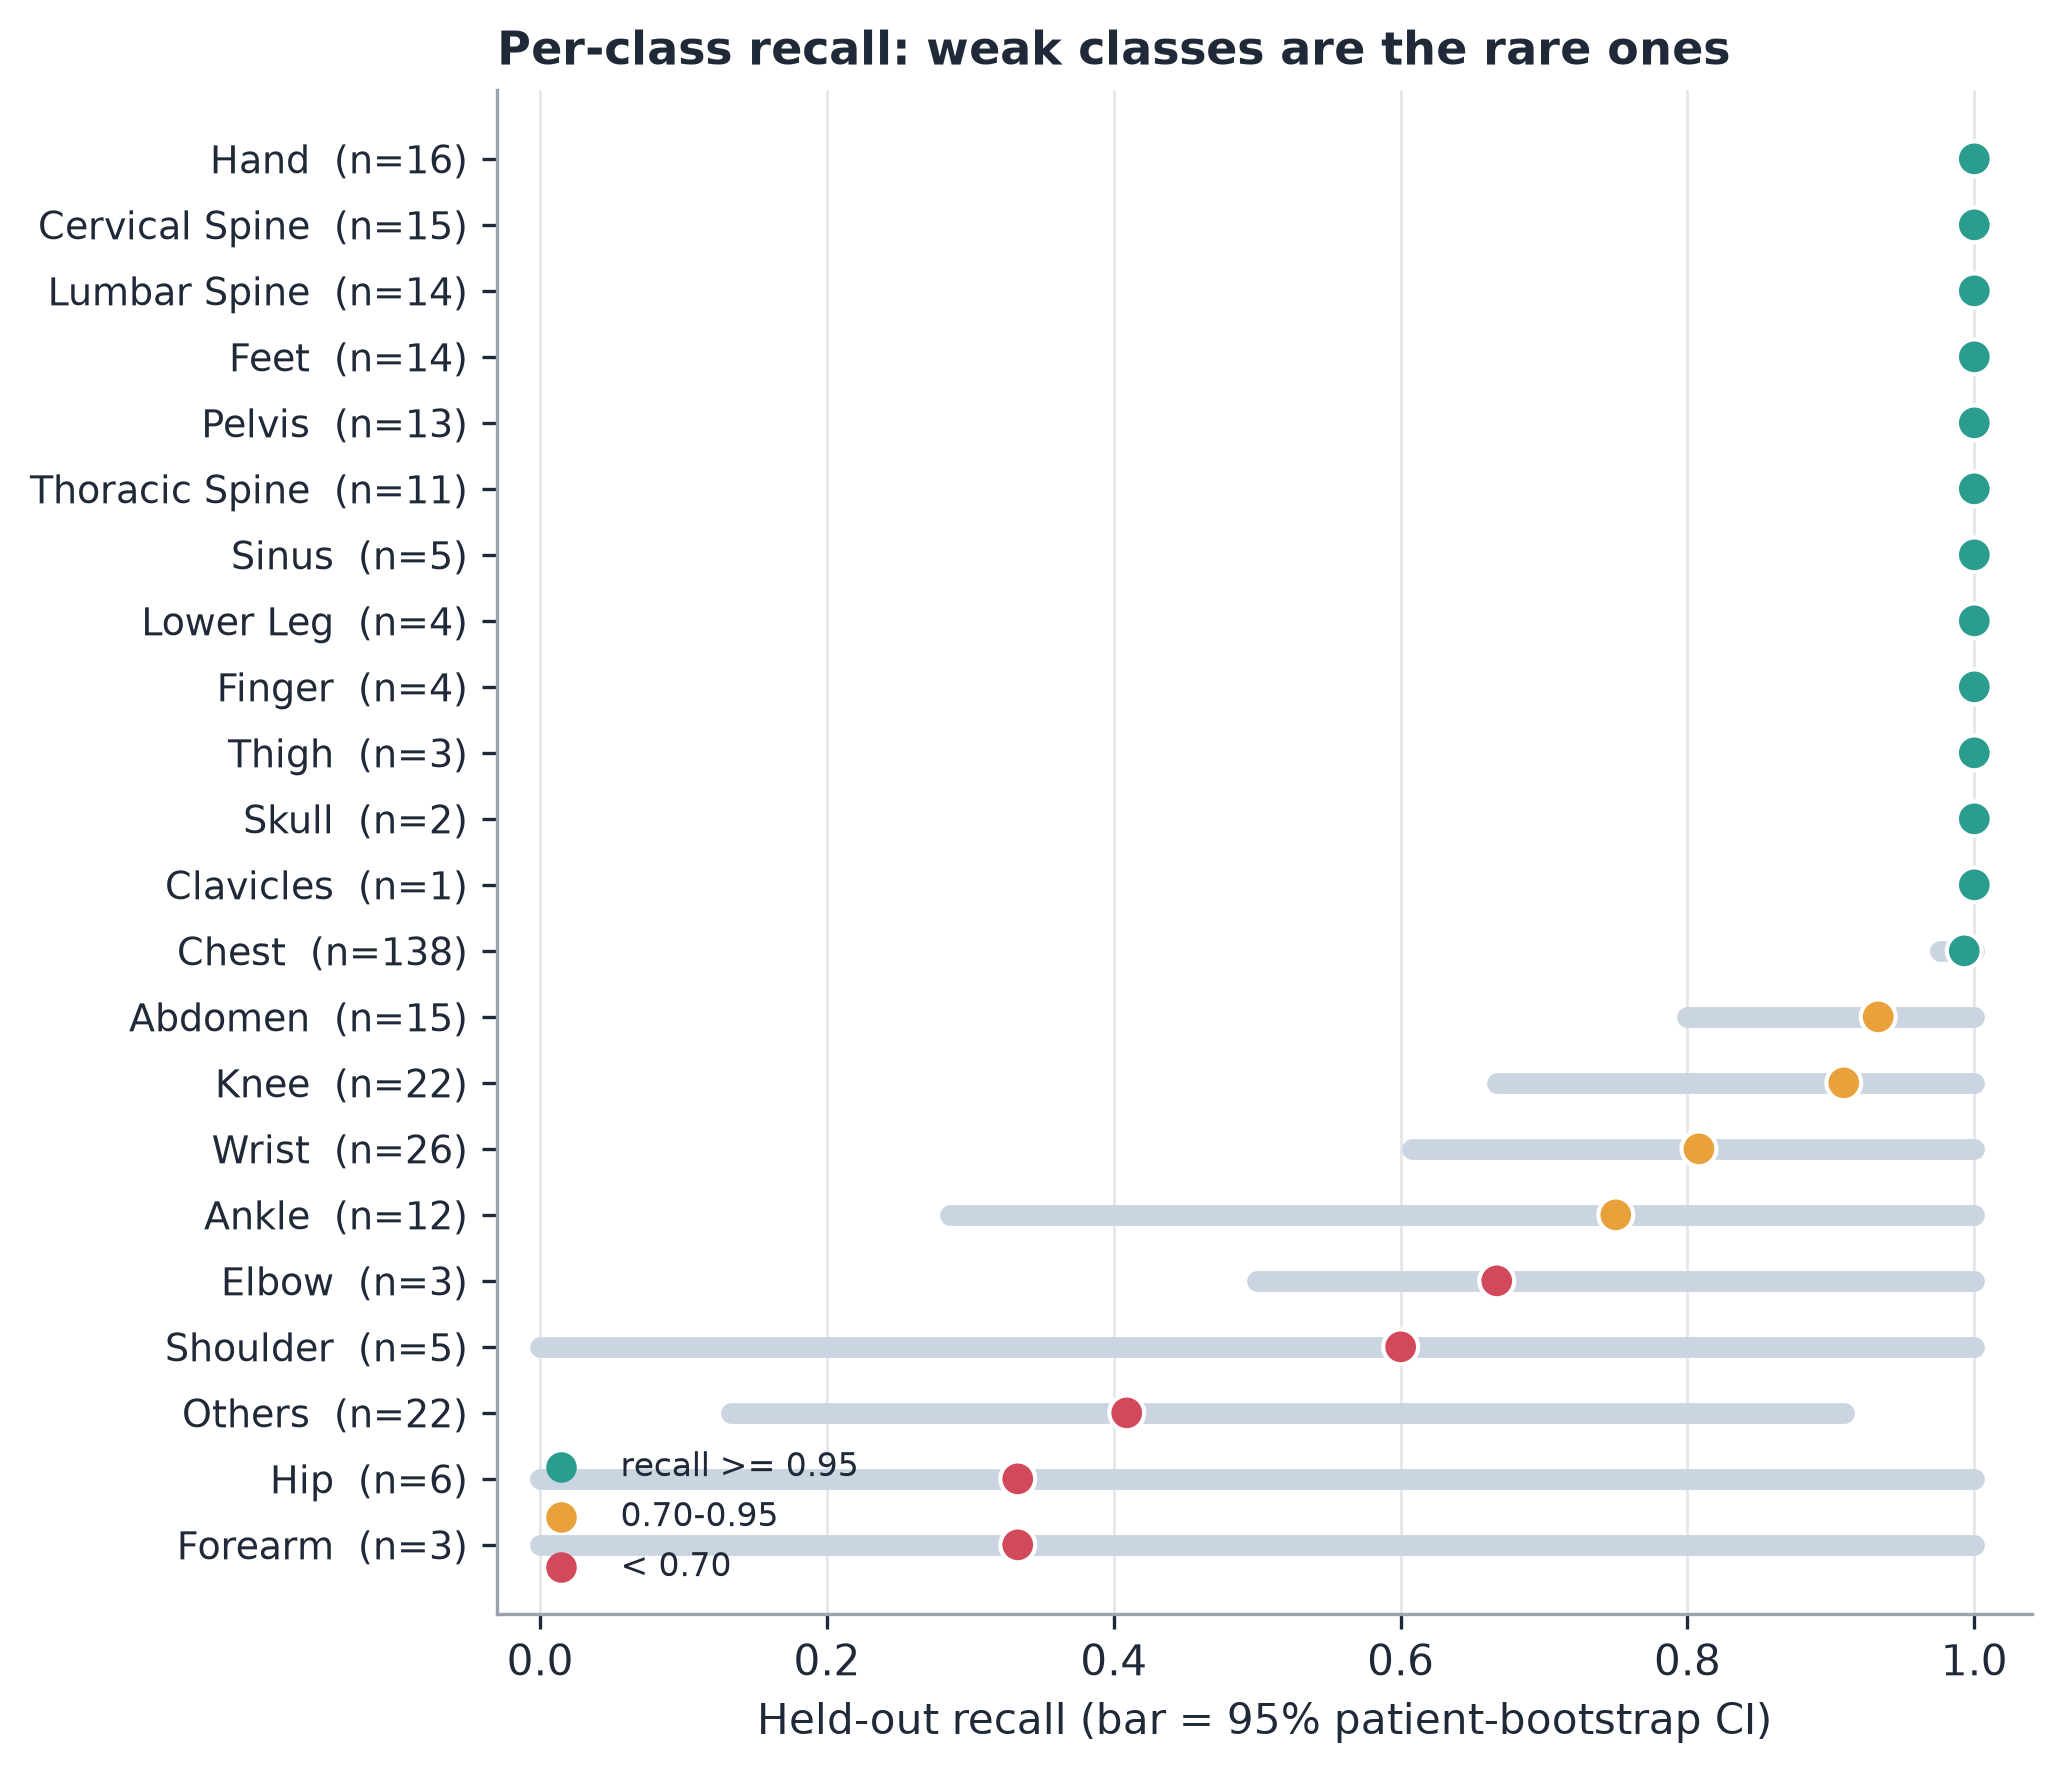
\includegraphics[width=0.85\textwidth]{figures/fig3_per_class_recall.png}\caption{Held-out recall for each class, with patient-bootstrap intervals. The weakest classes are also the rarest.}\label{fig:s1}\end{figure}
\end{document}
